\chapter{Implémentation des premiers réseaux}

Ce chapitre décrit l'implémentation de nos réseaux de neurones sous forme de perceptrons, que nous utiliserons par la suite dans les différentes applications. Nous verrons ici cette implémentation et le premier exemple avec le XOR.

\section{Implémentation du perceptron}

\subsection{Présentation et diagramme UML}

Comme décrit dans la partie théorique sur les perceptrons (1.5), nous avons choisi de représenter nos réseaux de neurones sous forme matricielle. Les neurones ne seront donc pas représentés individuellement, mais par couche de neurones (neuronLayer). Cela permet d'effectuer les calculs sous forme matricielle par rapport à des propagations et rétro-propagations neurone par neurone, ce qui fait gagner beaucoup de temps de calcul.
Cela est possible en gardant les mêmes fonctions d'activation pour chaque neurone d'une même couche, ainsi que les mêmes entrées et sorties. Dans le cadre du perceptron, cela convient.

Le diagramme UML comporte une classe principale, Application, qui va gérer les expériences et réseaux de neurones. Cette classe contient un réseau de neurones (NeuralNetwork) composé de plusieurs couches de neurones (NeuronLayer).Application possède aussi un collecteur quiest utilisé pour récupérer les données des expériences, les traiter et les exporter dans un fichier .csv. Enfin, la classe Teacher a pour rôle de gérer la rétropropagation et l'apprentissage du réseau de neurones.

\newpage

\begin{figure}[h]
\begin{center}
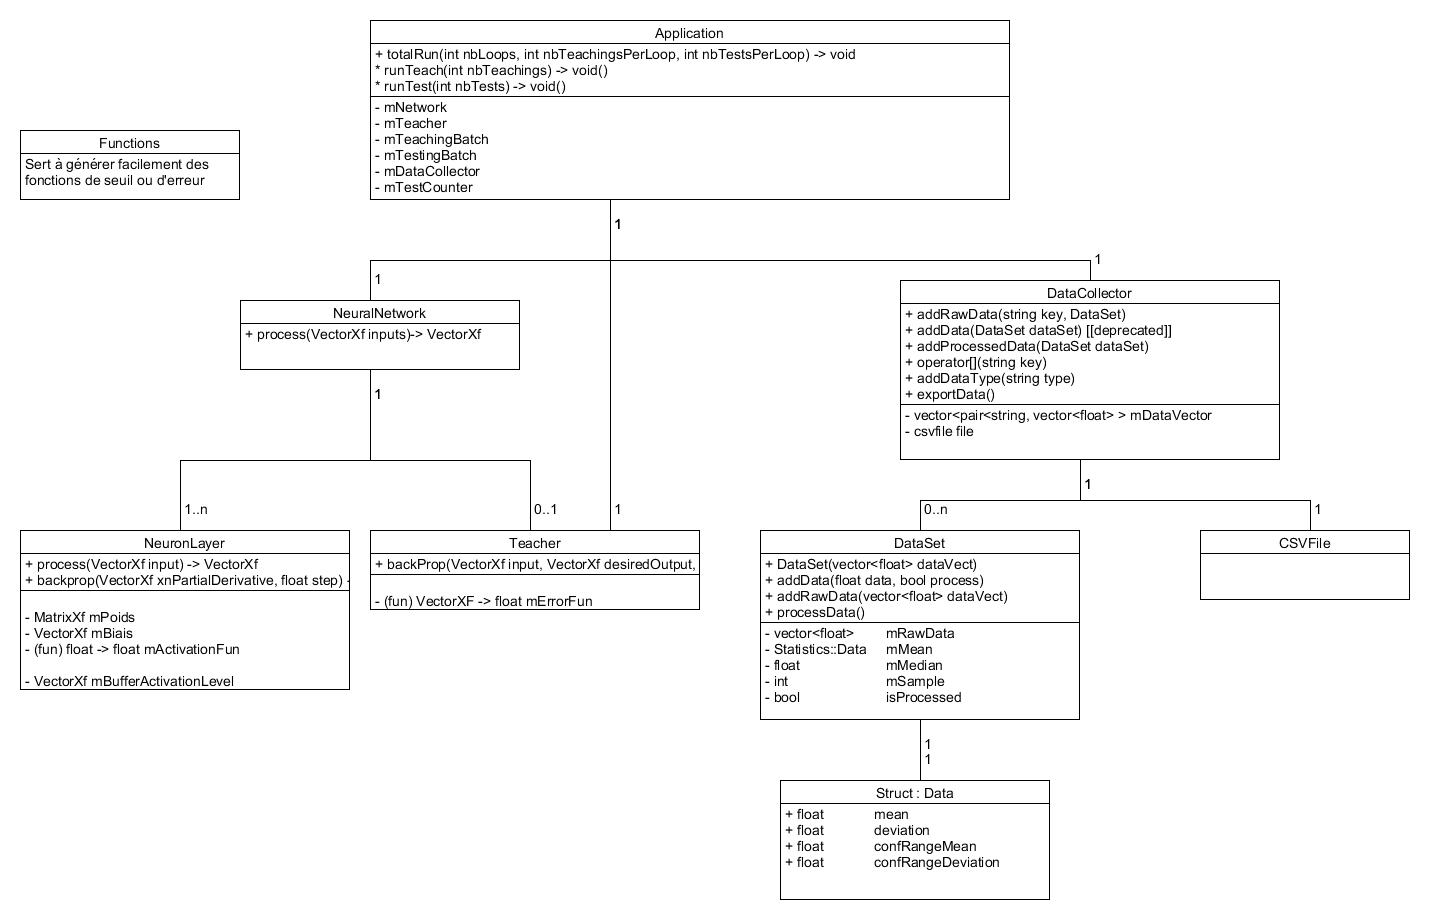
\includegraphics[width=1\textwidth]{images/umlDiagram.jpg}\caption{Diagramme UML}
\end{center}
\end{figure} 

\subsection{NeuralNetwork}

\subsection{DataCollector}

\section{Etude du XOR}